% Subsystem Report for the Analog Input Module system.
\fancyfoot[R]{WT}
\section[Analog Input]{Analog Input Module Subsystem}
\subsection{Description}
	The purpose of this subsystem is to scale the analogue input to an 
appropriate level so that it can be read by the analogue to digital converter.
The goal is to scale the output voltage to be between 0 and 5 volts and allow 
proper shifting and amplification via user interaction with the software. 
Circle 1 indicates where the input voltage is applied. The diode and resistor
 configuration allows the input range to be from -12.7 to +12.7. A reference 
voltage of + and -12 volts is used here and also supplies all the operation 
amplifiers. Circle 2 shows another voltage going into the inverting
 position of an op amp. This voltage is delivered through a digital to 
analogue converter. This allows the user to shift the voltage up or down. This
 voltage should range from 0 to +5 volts. Unable to test it with the micro 
controller, I directly used a voltage supply to simulate the voltage the 
digital to analogue converter would supply. The op amps by circles 1 and 2 
are voltage followers and act as buffers with the output equaling the input. 
The op amp by circle 5 acts as an inverting summer. Essentially the sum of the 
input voltage and voltage produced by the digital to analogue converter are 
summed together and inverted. It will also be amplified through the use of a 
multiplexer. Like the digital to analogue converter, the multiplexer gets 
information from the microcontroller and activates the desired output to use a 
resistor. These resistors, shown by circle 4, vary to allow for different
 levels of amplifications. For example, for 2x amplification, the 20k resistor 
is used (20k/10k = 2x amplification) and this is multiplied by the sum of the 
earlier voltages. The last op amp shown by figure 6 scales the signal to 
between 0 and 5 volts.
\begin{figure}[hbp]
\caption[Conditioner Schematic]{Schematic of Analog Input Module Signal Conditioner}
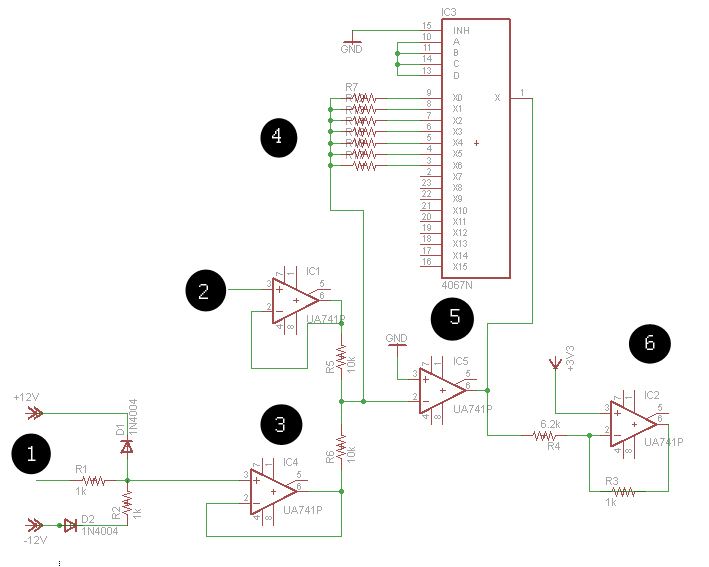
\includegraphics[width=5in]{sub_analog_sch.jpg}
\label{fig:analog schematic}
\end{figure}

\begin{figure}[hbp]
\caption{Photograph of implemented signal conditioner on breadboard}
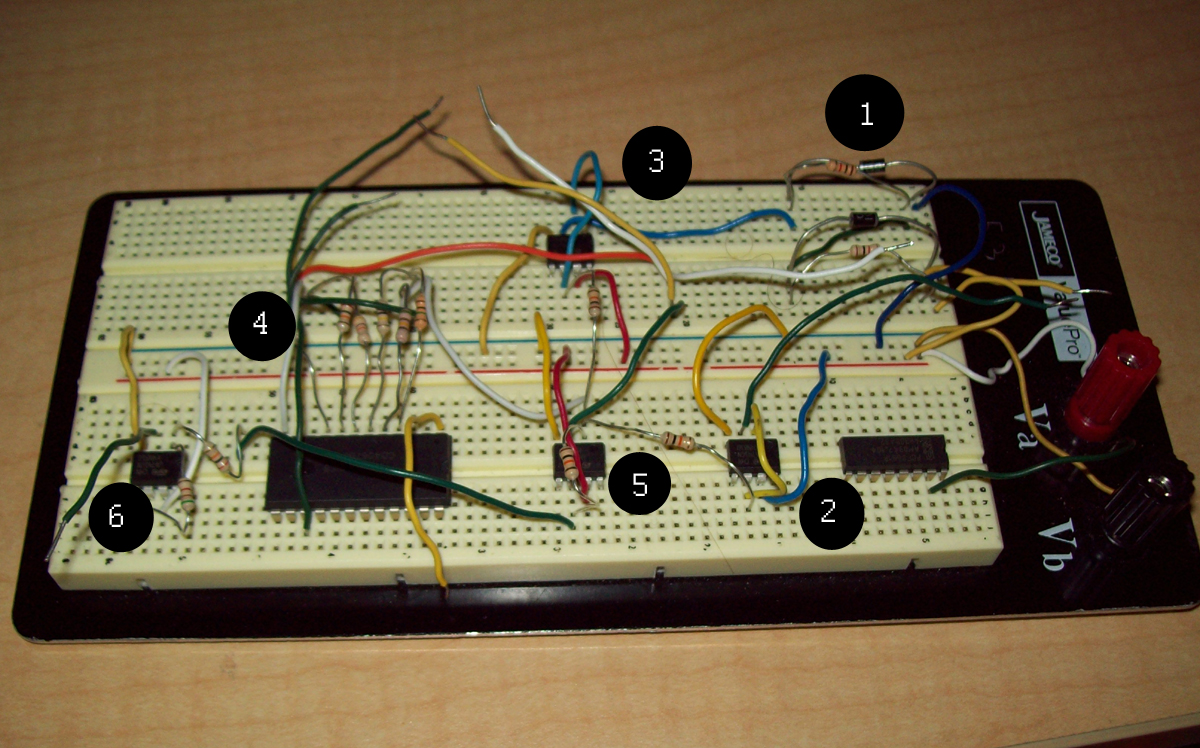
\includegraphics[width=5in]{sub_analog_hw.jpg}
\label{fig:analog breadboard}
\end{figure}

\subsection{Schedule of Implementation}
It took us a week at the most for our parts to arrive after ordering them from
 various companies. Building this circuit is straight forward and simple. It
 can easily be done within a day. The troubleshooting is where most of the
 time will take. It took me about 3 months of troubleshooting to get values
 that I was content with. Also, it could take longer depending if you test it
 with the micro controller or not. I would anticipate this would take a month
 to complete at the most to get it to perform ideally. The next paragraph 
describes my suggested technique to test the circuit after it is put together.

\subsection{Testing Notes}
Setting up the source voltages can be a little tricky. Since the 741 op amps 
are not rail to rail, the +12 and -12 reference voltages must be supplied using
 2 different voltage sources. If the circuit is going to be implemented 
separately from the microcontroller, another voltage source should be used as
 the voltage to the op amp by circle 2. Another voltage source of 3 volts
 should be applied to the noninverting input of the op amp by circle 6. 
Finally the input voltage should be applied to circle 1. I had trouble testing
 it initially with so many voltage sources, but I was able to find 2 triple
 power supply units to test it with. The feedback resistor of the op amp by 
circle 5 can be manually placed there instead of through the multiplexer if
 being tested without the micro controller. To test the circuit, I would first 
test to see if the voltage clamper works correctly by circle 1. Use a 
multimeter to test the voltage before op amp 3 and adjust the input to points 
outside the + and -12,7 volts. The output should not be bellow -12.7 nor
 above +12.7 volts. Next, I would test the op amps by circles 2 and 3 and make 
sure the output voltage is equal to the input. Then record the voltage coming 
out of the op amp by circle 5 with 10k feedback. This should be approximately 
equal to the inversion of the sum of the input and digital to analogue
 voltages.
\begin{equation}V = - [V_{DAC} + V_{IN}]\end{equation}
If this is correct, I would finally test the output voltage coming out of the op amp by circle 6. Put the input voltage to the max of 12.7 and the DAC voltage to its max of 5. This should yield an output of 0. Then set the input voltage to -12.7 and the DAC voltage to 0. The output voltage should be around 5 volts. Any other input voltage levels should show an output voltage between 0 and 5 and be approximately:
\begin{equation}V_{OUT} = 3 - .16447[V_{DAC} + V{IN}]\end{equation}

\subsection{Fault Analysis}
There are several obvious but overlooked reasons as to why this circuit would 
not operate properly. When I started off, I could not get any voltage out of 
an op amp I was using. I kept testing and asking for help and could not figure 
out what was wrong. Finally I moved the op amp to another part of the 
breadboard and it operated correctly right away. The breadboard was not
 working properly where I first placed the op amp. A faulty breadboard can be 
tested with a multimeter to make sure the connections are properly working.

It is possible to ruin your diodes or op amps if excess voltage is give to them.
If the diodes are facing the wrong direction they will also not operate 
properly. If there as any doubt of the components not working correctly, get 
new parts to replace them. The diodes and op amps are cheap so it won't cost 
very much to use another one.

If you are getting voltage values that are different than what the equation 
resulted in, it could be because of variances in each device. Make sure to use 
resistors with gold (5\%) tolerances. Also, you should measure the exact values
 before plugging them into the equations I used, not the theoretical values.

\subsection{Performance Data}
\begin{table}[hbp]
\caption[Test Results]{Testing Results (With 1x amplification)}
\begin{center}
\begin{tabular}{c| r @{.} l r @{.} l}  
	Input Voltage & \multicolumn{2}{r}{DAC Voltage} &
	\multicolumn{2}{r}{Output Voltage} \\ \hline
	12 & 7 & 5 & 1 & 4 \\ \hline
	10 & 0 & 3 & 3 & 2 \\ \hline
	-12 & 7 & 0 & 5 & 1 \\
\end{tabular}
\end{center}
\label{tab:analog input data}
\end{table}
